\documentclass[10pt]{article}
\usepackage{icmlko}

\icmlmeta{IP 파운데이션 월드모델}{158}{달력은 점수가 아니라 통제였다}{노트 157이 ``외부 축을 더 넣으면 부호가 좋아진다''고 예측했다. 반증됐다 --- 더 넣는 것이 아니라 달력 여섯이 전부를 하고, 그 여섯은 점수에는 안 보인다}

\begin{document}

\twocolumn[
\icmlheader

\begin{abstract}
노트 157이 검증 가능한 예측을 남겼다 --- ``외부 축은 통제 변수 노릇을 하니
더 넣으면 사전 부호 일치가 더 오른다.'' 확인하러 팝업에 위키 축을 붙였다
(한국어 위키, 덮음 60\%). 그리고 축을 다섯 → 아홉 → 열하나 → 열다섯 →
열아홉으로 늘려 가며 쟀다. \textbf{예측이 틀렸다.} 축 수와 부호 일치는
단조가 아니다. \textbf{달력 여섯이 전부를 한다.} 손 축 다섯만일 때 F18
배깅 72\% · F6 능형 58\%, 검색 넷을 더해도 \textbf{72\% · 58\%로 한 칸도
안 움직이고}, 달력 여섯을 더하면 \textbf{81\% · 78\%로 뛴다}(F6 은 20\%p).
그 위에 검색을 더해도, 위키를 더해도 81\% · 78\% 그대로다. 그래서 반대쪽을
쟀더니 \textbf{완벽하게 갈렸다.} 검색 넷은 판 $\rho$ 를 $+$0.069(F18) ·
$+$0.044(F6) 올리고 부호는 $+$0 이다. 달력 여섯은 판 $\rho$ 를
$+$0.012(F18) · \textbf{$-$0.038}(F6) --- 능형에서는 점수를 \emph{깎으면서}
부호를 20\%p 올린다. \textbf{두 무리가 서로 다른 일을 한다} --- 검색은
점수를 만들고 달력은 통제를 만든다. 이것이 오래 열려 있던 갈래 하나를 닫는다.
노트 130 이후 ``달력이 왜 트리에서만 되나''를 네 번 설명하려다 실패하고
관측으로 남겨 뒀는데, 물음이 틀렸던 것이다. \textbf{달력은 원래 점수 축이
아니다} --- 계절과 요일이 방문객을 움직이고 손 축이 계절과 얽혀 있으니,
달력을 안 넣으면 손 축이 그 교란을 대신 빨아들여 방향이 틀린다. 점수만
보는 순위표에서 달력은 거의 공짜로 보이고(F6 에서는 손해로 보이고),
\textbf{그 축의 값어치는 판정치에 원리적으로 안 나타난다.}
\end{abstract}
]

\begin{figure*}[t]
\centering
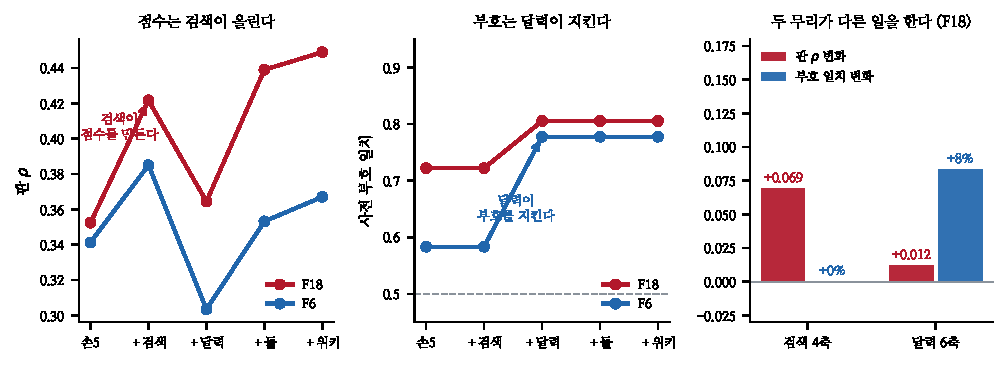
\includegraphics[width=\textwidth]{figs/ctrl.pdf}
\caption{왼쪽 --- 점수는 검색이 올린다. 가운데 --- 부호는 달력이 지킨다.
오른쪽 --- 두 무리가 다른 일을 한다.}
\end{figure*}

\section{예측이 틀렸다}

\begin{table}[t]
\centering\tsize
\caption{축을 늘려 가며. 사전 부호 일치(36칸 중).}
\begin{tabular}{lrr}
\toprule
& F18 배깅 & F6 능형 \\
\midrule
손5 (5축) & 72\% & 58\% \\
손5$+$검색 (9) & 72\% & 58\% \\
\textbf{손5$+$달력 (11)} & \textbf{81\%} & \textbf{78\%} \\
손5$+$검색$+$달력 (15) & 81\% & 78\% \\
전부 (19) & 81\% & 78\% \\
\bottomrule
\end{tabular}
\end{table}

\claimx{\textbf{축 수가 아니라 달력이다.} 검색 넷을 더해도 한 칸도 안
움직이고 달력 여섯을 더하면 뛴다. 그 위에 검색을 더하든 위키를 더하든
그대로다. \textbf{노트 157의 ``더 넣으면 좋아진다''는 반증됐다.}}{다섯
수준밖에 없어서 ``달력만''을 따로 못 봤다 --- 손 축 없이 달력만 두면 개입을
잴 축이 없다. 그래서 ``달력을 더하면''까지가 잰 것이다.}

\section{그래서 반대쪽을 쟀다}

\begin{table}[t]
\centering\tsize
\caption{손 축 다섯에 무엇을 더할 때의 변화.}
\begin{tabular}{lrrrr}
\toprule
& \multicolumn{2}{c}{F18 배깅} & \multicolumn{2}{c}{F6 능형} \\
& 판 $\rho$ & 부호 & 판 $\rho$ & 부호 \\
\midrule
\textbf{검색 4축} & \textbf{$+$.069} & $+$0 & \textbf{$+$.044} & $+$0 \\
\textbf{달력 6축} & $+$.012 & \textbf{$+$9\%p} & \textbf{$-$.038} & \textbf{$+$20\%p} \\
\bottomrule
\end{tabular}
\end{table}

\claimx{\textbf{완벽하게 갈린다.} 검색은 점수를 $+$0.069 올리고 부호는 하나도
안 고친다. 달력은 점수를 거의 안 올리거나(능형에서는 $-$0.038로 \emph{깎으면서})
부호를 9$\sim$20\%p 고친다.}{두 무리가 축 수도 다르고(4 대 6) 덮음도
다르다(검색은 도메인마다 0$\sim$98\%, 달력은 전부 100\%). 그 차이가 이
결과를 만들 수도 있다 --- 다만 방향이 이렇게 깨끗이 갈리는 것은 설명이
따로 필요하다.}

\section{오래 열려 있던 갈래 하나}

노트 130 이후 ``달력이 왜 트리에서만 되나''가 열린 채였다. 달력 축을 붙이면
F8 부스팅에서 판이 $+$0.010 오르는데 선형에서는 안 올랐고, 설명 넷을
시도했다가 다 실패해서 관측으로만 남겨 뒀다.

\claimx{\textbf{물음이 틀렸다.} 달력은 애초에 점수 축이 아니다. 계절과
요일이 방문객을 움직이고 손 축(굿즈 규모 · 미디어 푸시 · 입장 마찰)이
계절과 얽혀 있다 --- 여름 팝업과 연말 팝업은 기획이 다르다. 달력을 안
넣으면 손 축이 그 교란을 대신 빨아들이고, 계수가 커지는 대신 방향이
틀린다.}{그러면 ``트리에서만 판이 오른다''는 부수 현상이다 --- 트리는
계절 $\times$ 손 축 상호작용을 쓸 수 있고 선형은 못 쓴다. 값어치의 본체는
그 상호작용이 아니라 \textbf{교란 제거}다.}

\claimx{\textbf{그 값어치는 판정치에 원리적으로 안 나타난다.} 통제 변수는
점수를 올리라고 넣는 것이 아니다. 능형에서 달력이 판을 $-$0.038 깎으면서
부호를 20\%p 고치는 것이 정확히 그 모양이다. \textbf{순위표만 보면 달력은
빼야 할 축이다.}}{노트 148 · 155 · 156 · 157이 각각 다른 자리에서 같은
것을 가리켰다 --- 판 $\rho$ 하나로는 이 판의 절반이 안 보인다. 이 노트가
그 절반에 이름을 붙인다: \textbf{통제}.}

\section{덧 --- 팝업 위키}

예측을 확인하려고 팝업 메타의 IP 이름 376건으로 한국어 위키 조회수를
긁었다. 문서 매칭 60\%(45/75행)로 다른 도메인보다 높다. 자리표시자
이름(``미상'')이 한국어 위키에 실제 문서가 있어 정확 일치로 붙는 것을
잡아 막았다 --- 노트 150의 ``연애''와 같은 함정이다.

\begin{table}[t]
\centering\tsize
\caption{남은 것.}
\begin{tabular}{ll}
\toprule
\textbf{통제 축} & 달력 말고 또 무엇이 교란인가 --- 지역 · 요일 밖 \\
판정치 & 부호 일치를 순위표에 정식 열로 올린다 \\
달력 & 여섯 중 어느 것이 일하나 (주말? 월?) \\
\bottomrule
\end{tabular}
\end{table}

마지막 줄이 곧바로 잴 수 있다. 달력 여섯(요일 사인 · 코사인 · 주말 · 월
사인 · 코사인 · 공휴일 간격) 중 어느 것이 부호를 고치는지 하나씩 빼 보면
교란의 정체가 나온다. \textbf{그것이 다음 실험이다.}

\end{document}
